% Figure from MATH 591 notes, section 69. After the board (Lecture 25): the flow domain, time horizontal, with a flow box (user's figure).
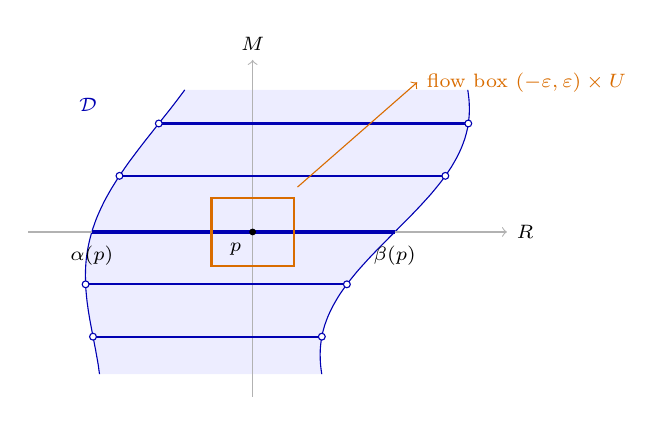
\begin{tikzpicture}[scale=0.95]
\fill[blue!7] plot[smooth] coordinates {(-2.047,-1.900) (-2.056,-1.836) (-2.065,-1.771) (-2.076,-1.707) (-2.088,-1.642) (-2.099,-1.578) (-2.112,-1.514) (-2.124,-1.449) (-2.137,-1.385) (-2.149,-1.320) (-2.161,-1.256) (-2.173,-1.192) (-2.184,-1.127) (-2.195,-1.063) (-2.204,-0.998) (-2.213,-0.934) (-2.220,-0.869) (-2.226,-0.805) (-2.231,-0.741) (-2.234,-0.676) (-2.235,-0.612) (-2.235,-0.547) (-2.233,-0.483) (-2.229,-0.419) (-2.223,-0.354) (-2.214,-0.290) (-2.204,-0.225) (-2.191,-0.161) (-2.176,-0.097) (-2.159,-0.032) (-2.140,0.032) (-2.118,0.097) (-2.095,0.161) (-2.069,0.225) (-2.040,0.290) (-2.010,0.354) (-1.978,0.419) (-1.943,0.483) (-1.907,0.547) (-1.868,0.612) (-1.828,0.676) (-1.787,0.741) (-1.743,0.805) (-1.699,0.869) (-1.653,0.934) (-1.605,0.998) (-1.557,1.063) (-1.508,1.127) (-1.458,1.192) (-1.408,1.256) (-1.357,1.320) (-1.306,1.385) (-1.255,1.449) (-1.204,1.514) (-1.153,1.578) (-1.102,1.642) (-1.052,1.707) (-1.003,1.771) (-0.954,1.836) (-0.907,1.900)} -- plot[smooth] coordinates {(2.876,1.900) (2.885,1.836) (2.892,1.771) (2.896,1.707) (2.897,1.642) (2.896,1.578) (2.891,1.514) (2.883,1.449) (2.872,1.385) (2.857,1.320) (2.839,1.256) (2.817,1.192) (2.792,1.127) (2.763,1.063) (2.731,0.998) (2.695,0.934) (2.657,0.869) (2.615,0.805) (2.570,0.741) (2.522,0.676) (2.471,0.612) (2.418,0.547) (2.363,0.483) (2.305,0.419) (2.246,0.354) (2.185,0.290) (2.123,0.225) (2.060,0.161) (1.996,0.097) (1.932,0.032) (1.868,-0.032) (1.804,-0.097) (1.740,-0.161) (1.677,-0.225) (1.615,-0.290) (1.554,-0.354) (1.495,-0.419) (1.437,-0.483) (1.382,-0.547) (1.329,-0.612) (1.278,-0.676) (1.230,-0.741) (1.185,-0.805) (1.143,-0.869) (1.105,-0.934) (1.069,-0.998) (1.037,-1.063) (1.008,-1.127) (0.983,-1.192) (0.961,-1.256) (0.943,-1.320) (0.928,-1.385) (0.917,-1.449) (0.909,-1.514) (0.904,-1.578) (0.903,-1.642) (0.904,-1.707) (0.908,-1.771) (0.915,-1.836) (0.924,-1.900)} -- cycle;
\draw[blue!70!black] plot[smooth] coordinates {(-2.047,-1.900) (-2.056,-1.836) (-2.065,-1.771) (-2.076,-1.707) (-2.088,-1.642) (-2.099,-1.578) (-2.112,-1.514) (-2.124,-1.449) (-2.137,-1.385) (-2.149,-1.320) (-2.161,-1.256) (-2.173,-1.192) (-2.184,-1.127) (-2.195,-1.063) (-2.204,-0.998) (-2.213,-0.934) (-2.220,-0.869) (-2.226,-0.805) (-2.231,-0.741) (-2.234,-0.676) (-2.235,-0.612) (-2.235,-0.547) (-2.233,-0.483) (-2.229,-0.419) (-2.223,-0.354) (-2.214,-0.290) (-2.204,-0.225) (-2.191,-0.161) (-2.176,-0.097) (-2.159,-0.032) (-2.140,0.032) (-2.118,0.097) (-2.095,0.161) (-2.069,0.225) (-2.040,0.290) (-2.010,0.354) (-1.978,0.419) (-1.943,0.483) (-1.907,0.547) (-1.868,0.612) (-1.828,0.676) (-1.787,0.741) (-1.743,0.805) (-1.699,0.869) (-1.653,0.934) (-1.605,0.998) (-1.557,1.063) (-1.508,1.127) (-1.458,1.192) (-1.408,1.256) (-1.357,1.320) (-1.306,1.385) (-1.255,1.449) (-1.204,1.514) (-1.153,1.578) (-1.102,1.642) (-1.052,1.707) (-1.003,1.771) (-0.954,1.836) (-0.907,1.900)}; \draw[blue!70!black] plot[smooth] coordinates {(0.924,-1.900) (0.915,-1.836) (0.908,-1.771) (0.904,-1.707) (0.903,-1.642) (0.904,-1.578) (0.909,-1.514) (0.917,-1.449) (0.928,-1.385) (0.943,-1.320) (0.961,-1.256) (0.983,-1.192) (1.008,-1.127) (1.037,-1.063) (1.069,-0.998) (1.105,-0.934) (1.143,-0.869) (1.185,-0.805) (1.230,-0.741) (1.278,-0.676) (1.329,-0.612) (1.382,-0.547) (1.437,-0.483) (1.495,-0.419) (1.554,-0.354) (1.615,-0.290) (1.677,-0.225) (1.740,-0.161) (1.804,-0.097) (1.868,-0.032) (1.932,0.032) (1.996,0.097) (2.060,0.161) (2.123,0.225) (2.185,0.290) (2.246,0.354) (2.305,0.419) (2.363,0.483) (2.418,0.547) (2.471,0.612) (2.522,0.676) (2.570,0.741) (2.615,0.805) (2.657,0.869) (2.695,0.934) (2.731,0.998) (2.763,1.063) (2.792,1.127) (2.817,1.192) (2.839,1.256) (2.857,1.320) (2.872,1.385) (2.883,1.449) (2.891,1.514) (2.896,1.578) (2.897,1.642) (2.896,1.707) (2.892,1.771) (2.885,1.836) (2.876,1.900)};
\draw[->, gray!60] (-3.0,0) -- (3.4,0) node[right, font=\scriptsize, text=black] {$\mathbb{R}$};
\draw[->, gray!60] (0,-2.2) -- (0,2.3) node[above, font=\scriptsize, text=black] {$M$};
\draw[blue!70!black, thick] (-2.134,-1.4) -- (0.925,-1.4); \draw[blue!70!black, fill=white] (-2.134,-1.4) circle (1.3pt); \draw[blue!70!black, fill=white] (0.925,-1.4) circle (1.3pt);
\draw[blue!70!black, thick] (-2.233,-0.7) -- (1.260,-0.7); \draw[blue!70!black, fill=white] (-2.233,-0.7) circle (1.3pt); \draw[blue!70!black, fill=white] (1.260,-0.7) circle (1.3pt);
\draw[blue!70!black, thick] (-1.780,0.75) -- (2.576,0.75); \draw[blue!70!black, fill=white] (-1.780,0.75) circle (1.3pt); \draw[blue!70!black, fill=white] (2.576,0.75) circle (1.3pt);
\draw[blue!70!black, thick] (-1.254,1.45) -- (2.883,1.45); \draw[blue!70!black, fill=white] (-1.254,1.45) circle (1.3pt); \draw[blue!70!black, fill=white] (2.883,1.45) circle (1.3pt);
\draw[blue!70!black, very thick] (-2.150,0) -- (1.900,0);
\fill (0,0) circle (1.3pt); \node[font=\scriptsize, anchor=north east] at (-0.02,-0.02) {$p$};
\node[font=\scriptsize, below] at (-2.150,-0.05) {$\alpha(p)$}; \node[font=\scriptsize, below] at (1.900,-0.05) {$\beta(p)$};
\draw[orange!85!black, thick] (-0.55,-0.45) rectangle (0.55,0.45);
\draw[->, orange!85!black] (0.6,0.6) -- (2.2,2.0) node[right, font=\scriptsize] {flow box $(-\varepsilon, \varepsilon) \times U$};
\node[font=\scriptsize, blue!70!black] at (-2.2,1.7) {$\mathcal{D}$};
\end{tikzpicture}
